\chapter{Architettura}

\section{Design Pattern Model-View-Presenter (MVP)}
Il pattern MVP separa le responsabilità in tre componenti distinti: il \textbf{Model}, che incapsula la business logic e la persistenza; la \textbf{View}, che agisce come interfaccia passiva delegando ogni decisione al Presenter; e il \textbf{Presenter}, che funge da orchestratore. A differenza del pattern MVC, la View non osserva direttamente il Model, riducendo l'accoppiamento e facilitando il testing in isolamento.

\begin{figure}[H]
    \centering
    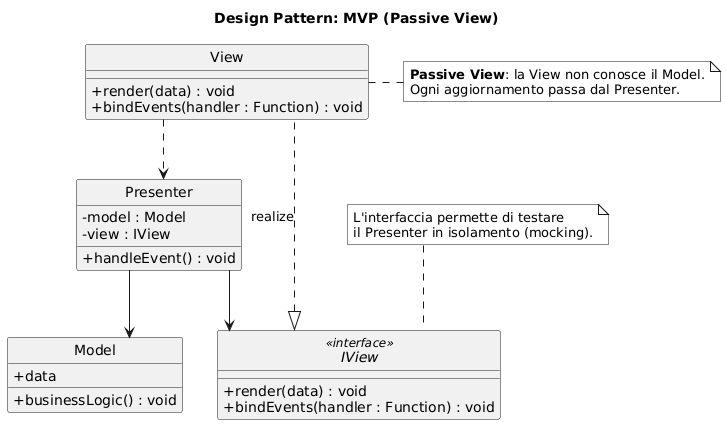
\includegraphics[width=0.8\textwidth]{DiagrammiDP/MVP.png}
    \caption{MVP}
    \label{fig:MVP}
\end{figure}

\subsection{Mapping nel codice}

\begin{itemize}
    \item \texttt{AppPresenter e AdminPresenter (Presenter)}: Fungono da mediatore; riceve gli input dalla View e coordina le richieste verso il Model, aggiornando l'interfaccia in base ai dati ricevuti.
    \item \texttt{AppModel (Model)}: Gestisce lo stato dei dati e l'interazione con le API REST del backend tramite richieste asincrone (\textit{Promises}).
    \item \texttt{BaseView, AppView, AuthView, AdminView, NoteView (View e IView)}: Rappresentano lo strato di visualizzazione (\textit{Passive View}); si occupano esclusivamente della manipolazione del DOM e del rendering dei corsi e degli appunti.
\end{itemize}

\section{Design Pattern Table Data Gateway}
Il pattern \textbf{Table Data Gateway} fornisce un oggetto che funge da gateway verso una specifica tabella del database. Esso contiene tutta la logica SQL \textit{(SELECT, INSERT, UPDATE, DELETE)} necessaria, isolando il resto dell'applicazione dai dettagli della persistenza. In genere restituisce un \textbf{RecordSet}, ovvero una struttura dati generica che mima la natura tabulare dei dati.

\begin{figure}[H]
    \centering
    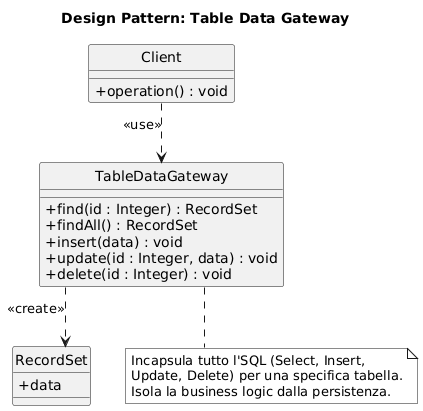
\includegraphics[width=0.6\textwidth]{DiagrammiDP/TDG.png}
    \caption{Table Data Gateway}
    \label{fig:TDG}
\end{figure}

\subsection{Mapping nel codice}

L'implementazione del sistema di persistenza segue una struttura gerarchica basata sul pattern \textbf{Table Data Gateway}, garantendo la separazione tra logica di business e accesso ai dati. Il mapping delle classi principali è articolato come segue:

\begin{itemize}
    \item \texttt{AbstractGateway} (Classe Base): Fornisce la logica comune a tutti i \textit{gateway}. Centralizza il metodo protetto \texttt{buildWhereClause()} il quale è fondamentale per trasformare i criteri astratti, definiti tramite il pattern \textit{Strategy}.
    
    \item \texttt{CoursesGateway}: Classe che gestisce la tabella \texttt{corsi}.
        
    \item \texttt{ArgomentiGateway}: Classe che gestisce la tabella \texttt{argomenti}.
    
    \item \texttt{NotesGateway}: Classe che gestisce la tabella \texttt{appunti}.
    
    \item \texttt{UserGateway}: Classe che gestisce la tabella \texttt{utenti}.
    
    \item \texttt{VersionsGateway}: Classe che gestisce la tabella \texttt{versioni}. Si occupa anche della persistenza degli stati storici degli appunti, interfacciandosi con il sistema di versionamento basato sul pattern \textit{Memento}.

\end{itemize}

\section{Design Pattern Strategy}
Il pattern \textbf{Strategy} è un pattern comportamentale utilizzato per definire una serie di algoritmi intercambiabili a runtime. Attraverso l'uso dell'aggregazione, il \textbf{Context} delega l'esecuzione del compito a un oggetto che realizza l'interfaccia \textbf{Strategy}.

\begin{figure}[H]
    \centering
    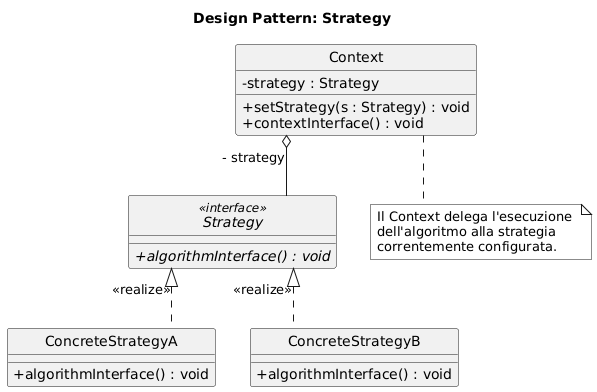
\includegraphics[width=0.8\textwidth]{DiagrammiDP/Strategy.png}
    \caption{Strategy}
    \label{fig:Strategy}
\end{figure}

\subsection{Mapping nel codice}

\begin{itemize}
    \item \texttt{FilterStrategy} (Interfaccia): \textit{Contratto} comune agli algoritmi di filtraggio. Definisce il metodo astratto \texttt{buildCriteria(QueryObject \$query)}, che obbliga ogni strategia concreta a popolare un oggetto di query con i criteri specifici del dominio.
    
    \item \texttt{CourseFilter}: Implementa il filtraggio degli argomenti in base all'identificativo di un corso specifico, in ottemperanza al requisito funzionale \textbf{RF4}.
    
    \item \texttt{ArgomentoFilter}: Filtro degli appunti in base all'identificativo di un argomento specifico.
    
    \item \texttt{SearchFilter}: Implementa la logica di ricerca testuale prevista dal requisito \textbf{RF9}. Istruisce il sistema a filtrare gli appunti il cui titolo corrisponde alla stringa inserita dall'utente tramite l'operatore SQL \texttt{LIKE} e l'utilizzo dei caratteri jolly \texttt{\%}.
    
    \item \texttt{IdFilter} e \texttt{EmailFilter}: Ulteriori specializzazioni del pattern utilizzate rispettivamente per recuperare il dettaglio di un singolo appunto (\textbf{RF5})o per estrarre le informazioni di un utente durante la procedura di \textit{login} tramite il campo \texttt{email} memorizzato nel database.

    \item \texttt{NoFilter}: Utilizzata per soddisfare il contratto \textbf{Strategy} quando non c'è bisogno di fare alcun filtro.

    \item \texttt{AppuntoFilter}: Permette di isolare le versioni appartenenti a uno specifico appunto, facilitando il recupero della cronologia (RF8).
    
    \item \texttt{IdInFilter}, \texttt{ArgomentiIdInFilter} e \texttt{AppuntoIdInFilter}: Strategie ottimizzate per la gestione di collezioni di identificativi tramite l'operatore \texttt{IN}. Sono componenti critici per il \texttt{CascadeService}, permettendo la rimozione atomica e sicura di record correlati in scenari di cancellazione massiva (RF10).

\end{itemize}

\section{Design Pattern Memento}

\noindent La gestione dello stato adotta il pattern \textbf{Memento}, garantendo l'incapsulamento dell'\texttt{Originator} tramite un'interfaccia ``stretta'' (\textit{narrow interface}). L'originatore crea i checkpoint mediante una \textit{Usage Dependency} (\guillemotleft\texttt{create}\guillemotright), mentre il \texttt{Caretaker} orchestra la cronologia dei dati. L'uso della molteplicità \texttt{[*]} per la proprietà \texttt{- history} assicura la gestione di una sequenza illimitata di stati, supportando operativamente l'\textit{undo} multi-livello.



\begin{figure}[H]
    \centering
    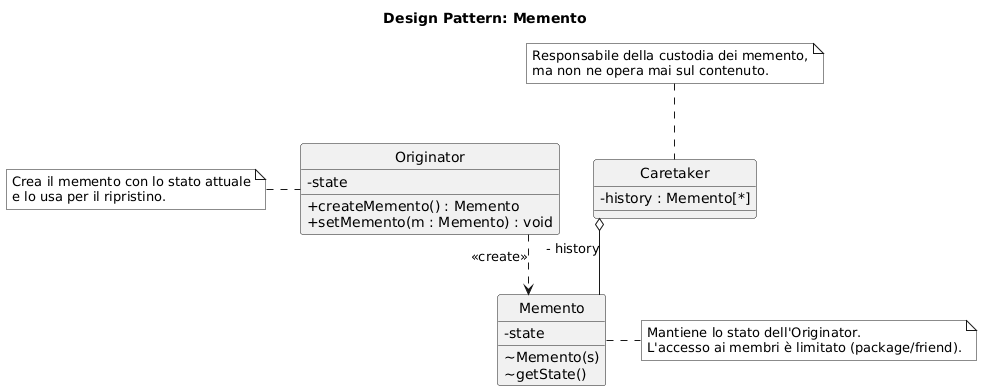
\includegraphics[width=1\textwidth]{DiagrammiDP/Memento.png}
    \caption{Memento}
    \label{fig:Memento}
\end{figure}


\subsection{Mapping nel codice}

\noindent L'implementazione del pattern \textbf{Memento} è distribuita tra le classi che gestiscono lo stato dell'appunto e lo strato di persistenza della cronologia:
\begin{itemize} 
    \item \texttt{Note}: Svolge il ruolo di \textit{Originator}. Detiene lo stato interno dell'appunto (testo, autore, ID) e implementa i metodi \texttt{saveToMemento()} per creare un'istantanea e \texttt{restoreFromMemento()} per il ripristino di uno stato precedente. 
    \item \texttt{NoteMemento}: Rappresenta l'oggetto \textit{Memento}. Incapsula i dati in modo immutabile e protegge l'incapsulamento fornendo lo stato tramite l'interfaccia stretta \texttt{getState()}, accessibile solo dall'Originator o dal Gateway di persistenza. 
    \item \texttt{VersionsGateway}: Agisce come \textit{Caretaker}. È l'unico componente responsabile della custodia fisica dei memento, gestendo la loro scrittura nel database (\texttt{saveVersion}) e il recupero dal file system. 
    \item \texttt{VersionController}: Coordina il flusso operativo, istruendo l'Originatore a generare il memento e delegando al Caretaker la sua conservazione all'interno di una transazione atomica. 
\end{itemize}

\section{Design Pattern Protection Proxy}

Il pattern Protection Proxy si configura come un'architettura di intermediazione in cui un oggetto $\texttt{Proxy}$ agisce da surrogato per un $\texttt{RealSubject}$, regolandone l'accesso in modo rigoroso. L'elemento cardine di tale struttura è l'astrazione definita dal $\texttt{Subject}$, che funge da contratto formale tra il sistema e il $\texttt{Client}$. Grazie a questo disaccoppiamento, il $\texttt{Client}$ interagisce esclusivamente con l'interfaccia astratta, ignorando se l'esecuzione avvenga tramite l'oggetto reale o il suo sostituto. Questa trasparenza operativa permette al sistema di evolvere e di integrare nuove logiche di sicurezza senza impattare minimamente sulle dipendenze esterne o sul codice chiamante.


\begin{figure}[H]
    \centering
    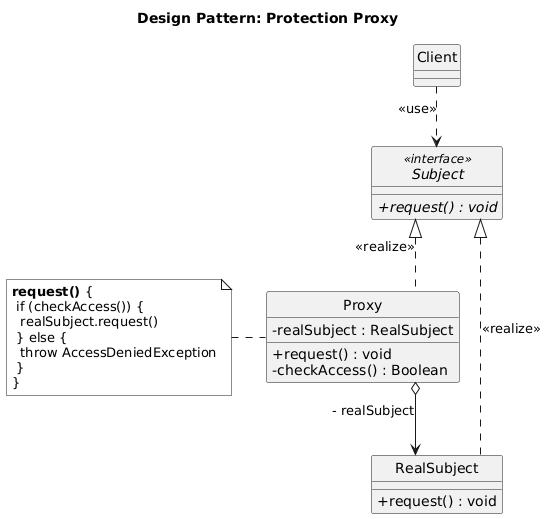
\includegraphics[width=0.8\textwidth]{DiagrammiDP/ProtectionProxy.png}
    \caption{Protection Proxy}
    \label{fig:ProtectionProxy}
\end{figure}


\subsection{Mapping nel codice}

\noindent La logica di sicurezza autoritativa è implementata tramite una serie di \textbf{Proxy} che filtrano l'accesso ai componenti di persistenza reale:
\begin{itemize} 
    \item \texttt{INotesGateway}, \texttt{IArgomentiGateway}, \texttt{IVersionsGateway}, \texttt{ICoursesGateway}: Definiscono l'interfaccia \textit{Subject}, che funge da contratto formale sia per il proxy che per il gateway reale, garantendo la trasparenza per il client (Controller). 
    \item \texttt{NotesGatewayProxy} e \texttt{VersionsGatewayProxy}: Implementano il ruolo di \textit{Proxy} per le risorse dinamiche. Intercettano le chiamate a metodi sensibili (come \texttt{createNote} o \texttt{saveVersion}), verificano il ruolo \texttt{studente} e negano l'accesso in caso di privilegi insufficienti.
    \item \texttt{NotesGateway}, \texttt{ArgomentiGateway}, \texttt{CoursesGateway} e \texttt{VersionsGateway}: Rappresentano i \textit{RealSubject}. Contengono la logica SQL (\texttt{PDO}) effettiva e la gestione del file system. Vengono invocati dai rispettivi proxy solo dopo il superamento con successo dei controlli autoritativi.
    \item \texttt{CoursesGatewayProxy} e \texttt{ArgomentiGatewayProxy}: Specializzazioni del proxy che proteggono la struttura del catalogo, riservando le operazioni di modifica ed eliminazione esclusivamente agli utenti con ruolo \texttt{amministratore}. 
\end{itemize}
